\documentclass{beamer}

\usepackage[utf8]{inputenc}
\usepackage{amsmath}
\usepackage{algorithm}
\usepackage{algpseudocode}

\title{A Tutorial on Multigrid Methods}
\author{Philip Greggory Lee}
\institute{
 Electrical Engineering and Computer Science\\
 Northwestern University\\
 Evanston, IL 60208
}

\AtBeginSection
{
 \begin{frame}{Outline}
  \tableofcontents[currentsection]
 \end{frame}
 \addtocounter{framenumber}{-1}
}

\providecommand{\defeq}{\stackrel{\Delta}{=}}
\providecommand{\abs}[1]{\left\lvert #1 \right\rvert}
\providecommand{\norm}[1]{\left\lVert #1 \right\rVert}

\begin{document}

\begin{frame}
 \titlepage
\end{frame}

\begin{frame}{Copyright 2013 Philip G. Lee}
 \begin{center}
 Permission is granted to copy, distribute and/or modify this document
 under the terms of the GNU Free Documentation License, Version 1.3
 or any later version published by the Free Software Foundation;
 with no Invariant Sections, no Front-Cover Texts, and no Back-Cover Texts.
 A copy of the license is included in the file \texttt{COPYING.GFDL.tex}.
 \end{center}
\end{frame}

\begin{frame}{Outline}
 \tableofcontents
\end{frame}
\addtocounter{framenumber}{-1}

\section{Introduction}%========================================================

\begin{frame}{The Problem}
 \begin{itemize}
  \item Suppose we have a linear system whose variable $u$ represents a discretization
        of a function $g(x)$ on a regular grid.
  \begin{align}
   Au=f
  \end{align}
  \item As the level of discretization grows, so does the size of the system.
  \item In many typical cases, the condition number of $A$ grows with the
        square of the size of $u$.
  \item Simple linear solvers therefore slow down dramatically as the resolution
        increases.
 \end{itemize}
\end{frame}

\begin{frame}{The Intuition}
 \begin{itemize}
  \item Why should this be the case?
  \item In most cases, increasing the resolution does not \textit{really}
        introduce more complexity into the problem.
  \item Is there any way we can take advantage of the notion of
        \textit{resolution} of the solution $u$ in a principled way?
  \item The answer is yes, and we will explore a class of ways to do so called
        \textbf{multigrid methods}.
 \end{itemize}
\end{frame}

\section{The Motivating Example}%==============================================

\begin{frame}{1D Laplace Problem I}
 \begin{itemize}
  \item A simple example that serves to illustrate the major points of this
        tutorial is the Laplace equation in 1D with Dirichlet boundary
        conditions.
  \begin{align}
   Au &= f, \; \text{where} \label{eq:laplace} \\
   Au &= -\Delta u = - \nabla \cdot \nabla u, \; \text{and} \nonumber \\
   f &= 0 \nonumber \\
   \text{s.t.} \; & u_0 = u_{n+1} = 0 \nonumber
  \end{align}
  \item There are $n$ free variables $u_1,\dotsc,u_n$, and $A$ is $n \times n$.
  \item In this case, the Laplace operator $\Delta$ can be represented by
        convolution with the kernel $[1,-2,1] = [1,-1]\ast[1,-1]$.
 \end{itemize}
\end{frame}

\begin{frame}{1D Laplace Problem II}
 \begin{figure}
  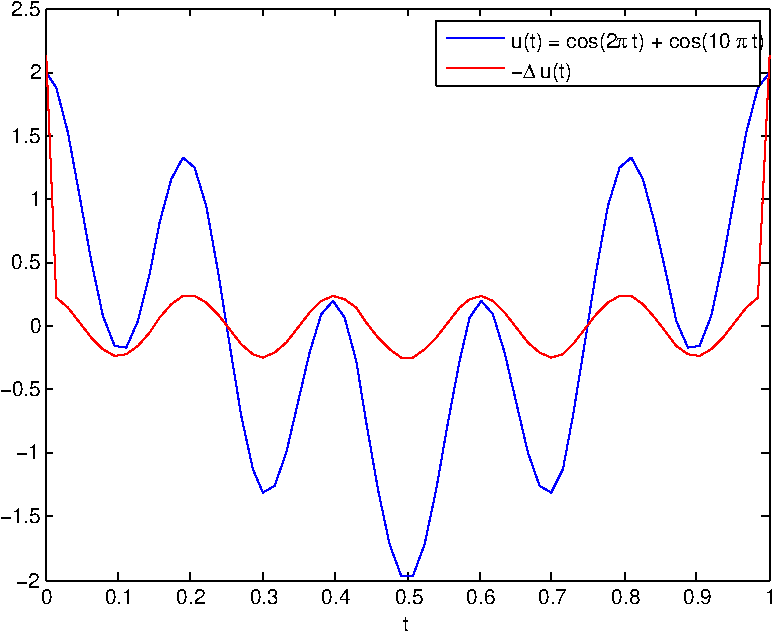
\includegraphics[width=6cm]{images/laplaceOperatorExample.pdf}
 \end{figure}
 \begin{itemize}
  \item Strictly speaking, if we are approximating the continuous Laplace
        operator, then the kernel is $\frac{1}{h^2}[1,-2,1]$ if the samples
        are spaced $h$ units apart. It's just a scaling factor.
  \item For simplicity, we will assume that the discrete variables are spaced
        $h = 1/(n+1)$ units apart so that $u$ represents a function over the
        unit interval $[0,1]$.
 \end{itemize}
\end{frame}

\begin{frame}{1D Laplace Problem III}
 \begin{itemize}
  \item Equation $i$ of \eqref{eq:laplace} reads:
  \begin{align}
   -u_{i-1}+2u_i-u_{i+1} = 0, \; \forall 1 \leq i \leq n
  \end{align}
  \item Notice that the boundary conditions $u_0 = u_{n+1} = 0$ are incorporated
        into this system.
  \item In this particular case, the eigenfunctions of A are $v^h_{(k)i} = \sin(k \pi ih)/h$,
        with $1 \leq i,k \leq n$ and its eigenvalues range from $\lambda_1^h \approx \pi^2 h^2$ to
        $\lambda_n^h \approx 4-h^2$.
  \item $\lambda_i^h = 2-2\cos( i\pi h )$
  \item Notice that the condition number
        $\kappa(A) = \lambda_n^h / \lambda_1^h \approx 4/(\pi^2h^2) = 4(n+1)^2/\pi^2$.
  \item So, the condition number grows as $O(n^2)$ with system size $n$.
  \item We will see that this is the major problem facing standard linear solvers.
 \end{itemize}
\end{frame}

\begin{frame}{1D Laplace Problem IV}
 \begin{figure}
  \begin{tabular}{cc}
   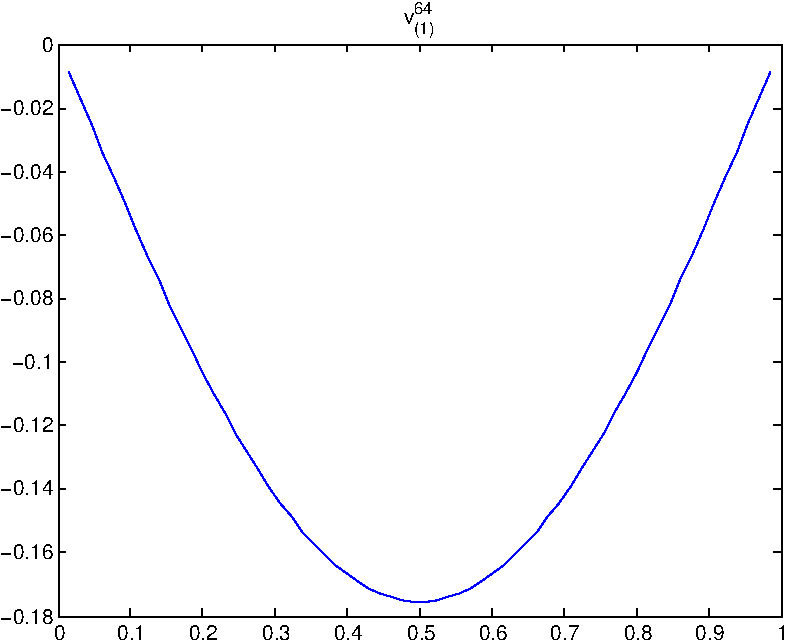
\includegraphics[width=4cm]{images/v64_1.pdf} & 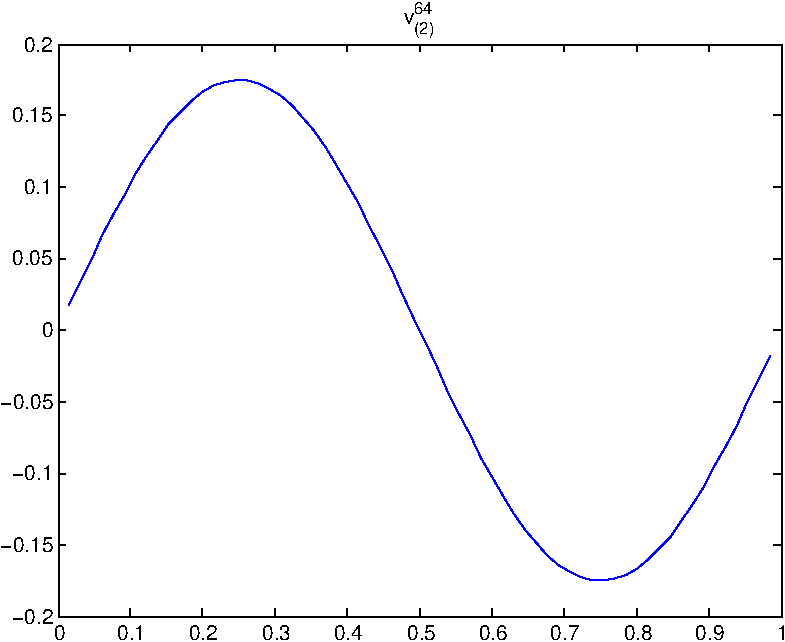
\includegraphics[width=4cm]{images/v64_2.pdf} \\
   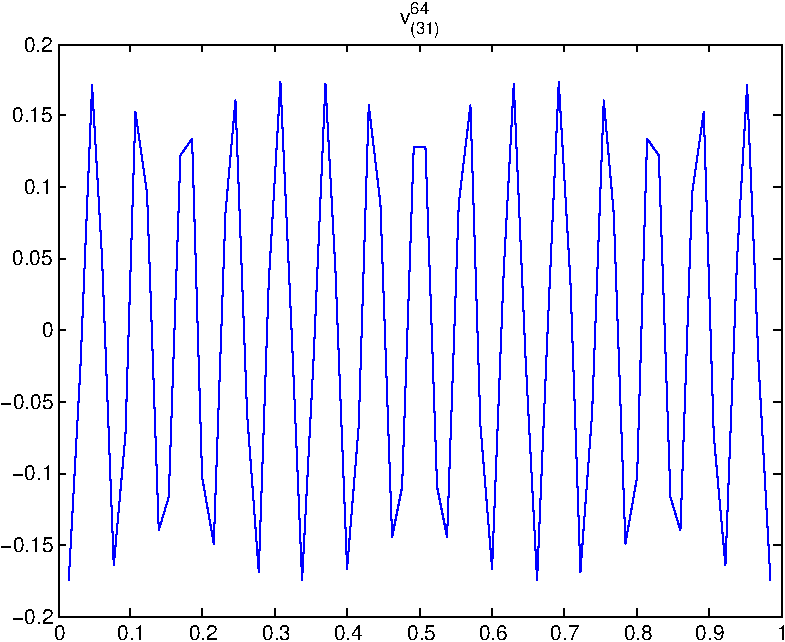
\includegraphics[width=4cm]{images/v64_31.pdf} & 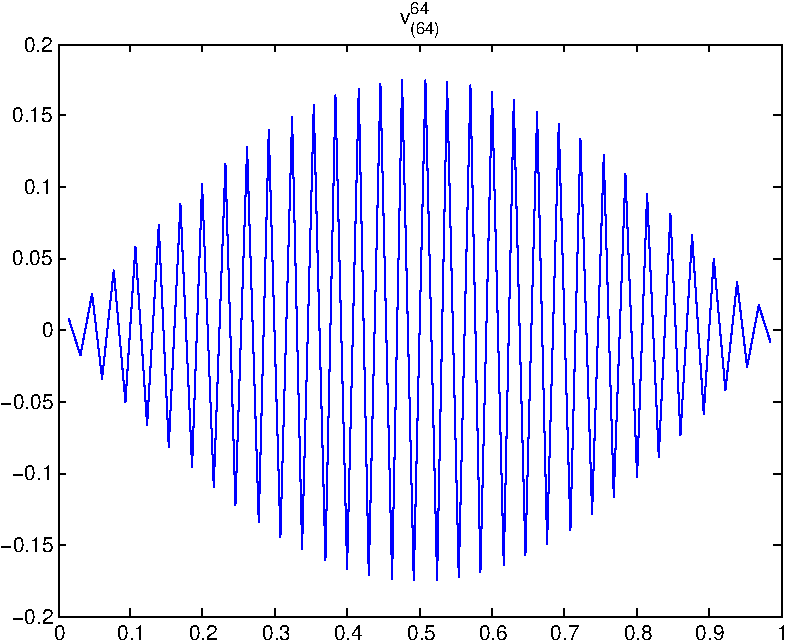
\includegraphics[width=4cm]{images/v64_64.pdf}
  \end{tabular}
  \caption{Eigenfunctions of $A$ when $n=64$ ($h=1/65$).}
 \end{figure}
\end{frame}

\section{Relaxation (Iterative Methods)}%======================================

\begin{frame}{Jacobi Method}
 \begin{itemize}
  \item How can we solve such a problem?
  \item A first stab is just to satisfy each equation independently:
  \begin{align}
   u_{i(\text{new})} \leftarrow \frac{u_{i-1}+u_{i+1}+f_i}{2}
  \end{align}
  \item \textbf{Remember}: for us, $f_i=0$.
  \item This is the strategy of the \textbf{Jacobi Method}.
  \item Formally, if $D$, $-L$, and $-U$ are the diagonal, lower, and upper
        triangular parts of $A$ resp., then $A=D-L-U$ and the Jacobi Method is:
  \begin{align}
   u \leftarrow D^{-1}(L+U)u+D^{-1}f
  \end{align}
 \end{itemize}
\end{frame}

\begin{frame}[label=relaxation1]{Relaxation I}
 \begin{itemize}
  \item In general, we call any method of the following form \textbf{relaxation}:
  \begin{align}
   u \leftarrow G(u) = Ru+g.
  \end{align}
  \item If $\hat{u}$ is the solution, it must be the case that it is a fixed
        point of the iteration: $\hat{u} = R\hat{u}+g$.
  \item For analysis, it is useful to make the transformation
  \begin{align}
   e &\defeq \hat{u}-u \nonumber \\
   r &\defeq f-Au \nonumber
  \end{align}
  \item This means the original problem is transformed to $Ae=r$.
 \end{itemize}
\end{frame}

\begin{frame}{Relaxation II}
 \begin{itemize}
  \item Note that $\hat{e} = 0$.
  \begin{align}
   e_{\text{new}} &= \hat{u} - (Ru+g) \nonumber \\
                  &= \hat{u} - R(\hat{u}-e) - g \nonumber \\
                  &= \hat{u} - (\hat{u}-g) + Re - g \nonumber \\
                  &= Re
  \end{align}
  \item So, $e_\text{new} = Re$, written in algorithmic form as $e \leftarrow Re$.
  \item The eigenvalue equation gives $\norm{e_\text{new}}_2 \leq \rho(R)\norm{e}_2$, or
  \begin{align}
   \frac{\norm{e_{\text{new}}}_2}{\norm{e}_2} \leq \rho(R).
  \end{align}
  \item After $k$ iterations, $\norm{e_k}_2/\norm{e_0}_2 \leq [\rho(R)]^k$.
  \item Since this iteration must converge to 0, a sufficient condition for
        convergence is $\rho(R) < 1$.
 \end{itemize}
\end{frame}

\begin{frame}{Jacobi Convergence Rate I}
 \begin{itemize}
  \item Note that for the Jacobi method, the iteration matrix $R=D^{-1}(L+U)$.
  \item What is $\rho(R)$?
  \item We will prove that $\rho(R) \leq 1-\frac{\pi^2 h^2}{2}$
 \end{itemize}
\end{frame}

\begin{frame}{Jacobi Convergence Rate II}
 \begin{theorem}
  $\rho(R) \leq 1-\frac{\pi^2 h^2}{2}$
   
  \begin{proof}
   Proof by contradiction. Suppose $\exists y$ s.t. $Ry = (1-\frac{\pi^2 h^2}{2}+\epsilon)y$.
   Then,
   \begin{align}
    Ay &= (D-DR)y = Dy-DRy \nonumber \\
       &= 2y - 2(1-\frac{\pi^2 h^2}{2}+\epsilon)y \nonumber \\
       &= (\pi^2 h^2 - 2 \epsilon) y
   \end{align}
   So, $y$ is an eigenfunction of $A$ with eigenvalue $\pi^2 h^2 - 2 \epsilon$.
   But this is a contradiction since $\lambda^h_1 = \pi^2 h^2$.
  \end{proof}
 \end{theorem}
\end{frame}

\begin{frame}{Jacobi Convergence Rate III}
 \begin{itemize}
  \item So, using the Jacobi method, the convergence rate slows quadratically
        with $n$.
  \begin{figure}
   \begin{tabular}{cc}
    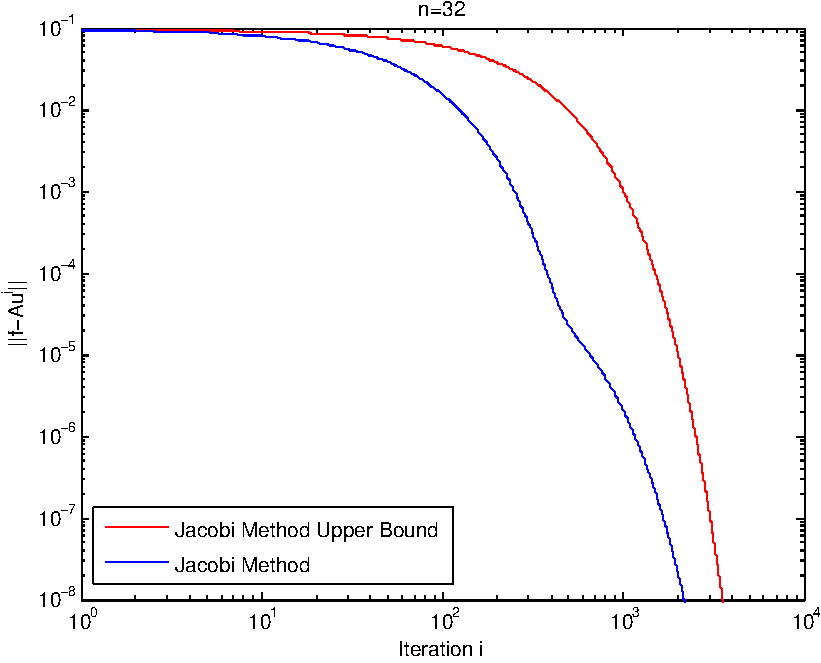
\includegraphics[width=4.5cm]{images/jacobiConvergence_32.pdf} & 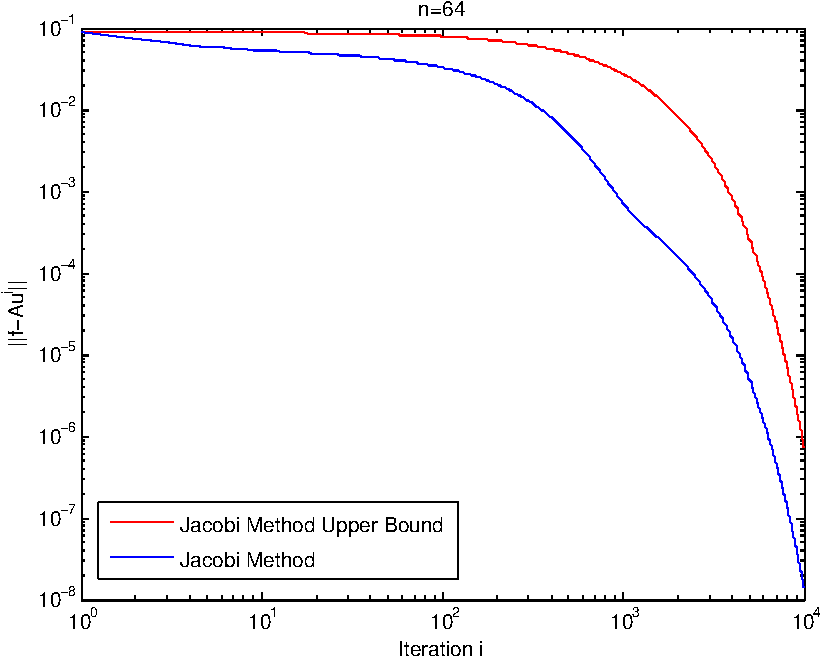
\includegraphics[width=4.5cm]{images/jacobiConvergence_64.pdf}
   \end{tabular}
   \caption{Convergence rate and upper bound for convergence rate of Jacobi
            method on our model problem.}
  \end{figure}
  \item In fact, the eigenvalues of $R$ range from $\mu_1^h \approx 1-\pi^2h^2/2$
        to $\mu_n^h \approx -\mu_1^h$.
 \end{itemize}
\end{frame}

\begin{frame}{Jacobi Convergence Rate IV}
 \begin{itemize}
  \item \textbf{Important}: notice that low-frequency eigenfunctions ($i\ll n$)
        of $A$ correspond to $\mu_i \approx 1$ and high-frequency eigenfunctions
        ($i \approx n$) correspond to $\mu_i \approx -1$.
  \item This means that very high and very low frequency components of error $e$
        are very slow to converge.
  \item On the flip side, mid-frequency components correspond to
        $\mu_i \approx 0$ and converge very quickly indeed.
  \item To see why, notice we can decompose $e = \sum_i a_i v_i$, where $v_i$
        are the eigenfunctions of $R$.
  \item Then, after $k$ iterations, $\norm{e} = \norm{\sum_i a_i \mu_i^k v_i} \leq \abs{a_1\mu_1^k} + \abs{a_n\mu_n^k} + O(\abs{\mu_2^k})$
  \item We can also see that the $i^\text{th}$ frequency component converges
        geometrically like $\mu_i^k$.
 \end{itemize}
\end{frame}

\begin{frame}{Jacobi Convergence Rate V}
 \begin{figure}
  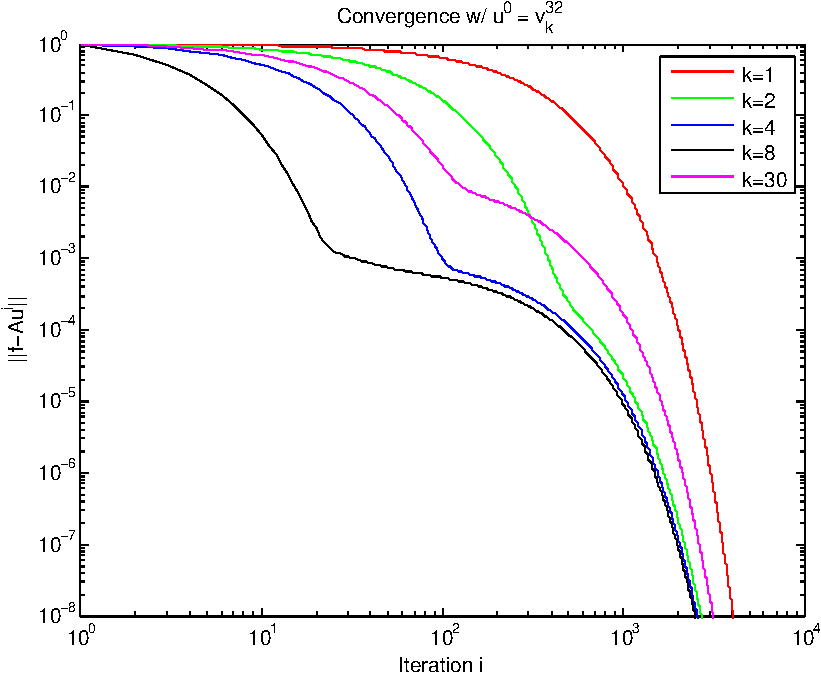
\includegraphics[width=6cm]{images/jacobiConvergence_freq.pdf}
  \caption{$n=32$. High and low-frequency components ($k \approx 1$ or
           $k \approx 32$) converge slowly, while mid-frequency components
           converge quickly.}
 \end{figure}
\end{frame}

\begin{frame}[label=gaussSeidel]{Gauss-Seidel}
 \begin{itemize}
  \item Another simple relaxation method is \textbf{Gauss-Seidel}.
  \item Instead of always using the old values of $u$ to get $u_{(\text{new})}$,
        it uses the new values immediately after computing them to solve each
        equation.
  \begin{align}
   u_{i\text{(new)}} \leftarrow \frac{u_{i-1\text{(new)}}+u_{i+1}+f_i}{2}
  \end{align}
  \item In operator notation, this is
  \begin{align}
   u \leftarrow (D-L)^{-1}Uu + (D-L)^{-1}f
  \end{align}
  \item So, the iteration matrix in this case is $R_G=(D-L)^{-1}U$.
  \item It turns out that $\rho(R) \leq \left[\rho(R_J)\right]^{2}$.
  \item So, it converges twice as fast as the Jacobi method.
  \item For the proof, see
        \hyperlink{gaussSeidelProof}{\beamergotobutton{GS Spectrum Proof}}
 \end{itemize}
\end{frame}

\begin{frame}{Gauss-Seidel Spectrum I}
 \begin{itemize}
  \item Unlike the Jacobi matrix, the eigenfunctions of the Gauss-Seidel matrix
        are not pure sinusoids, but still go from ``low frequency'' to
        ``high frequency''.
 \end{itemize}
 \begin{figure}
  \begin{tabular}{cc}
   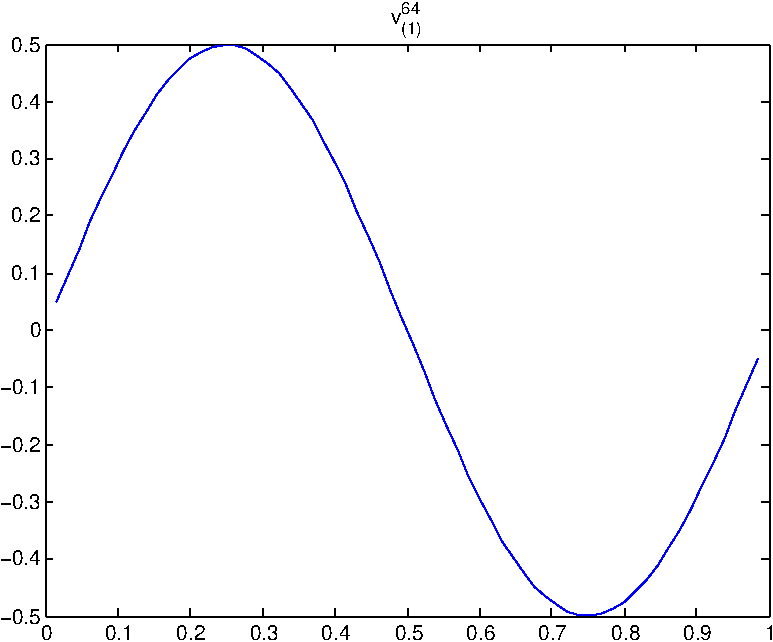
\includegraphics[width=3cm]{images/gauss_v64_1.pdf} & 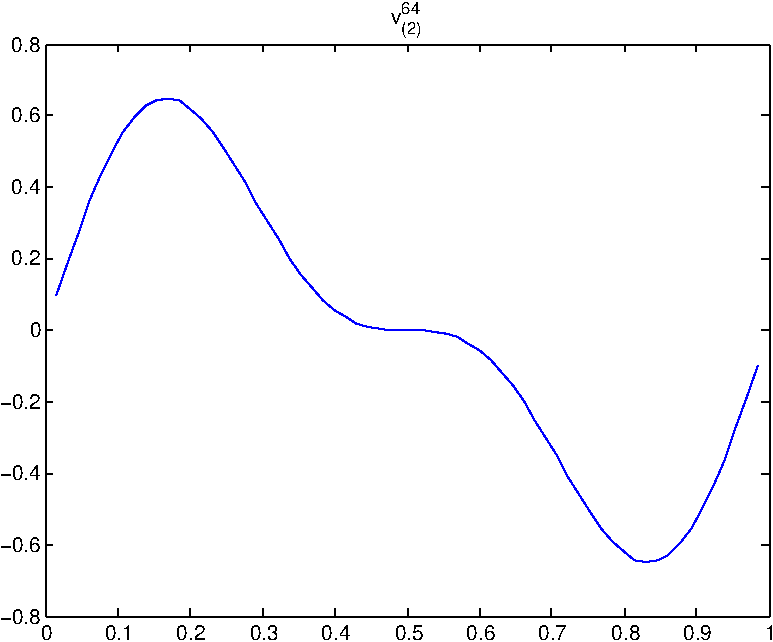
\includegraphics[width=3cm]{images/gauss_v64_2.pdf} \\
   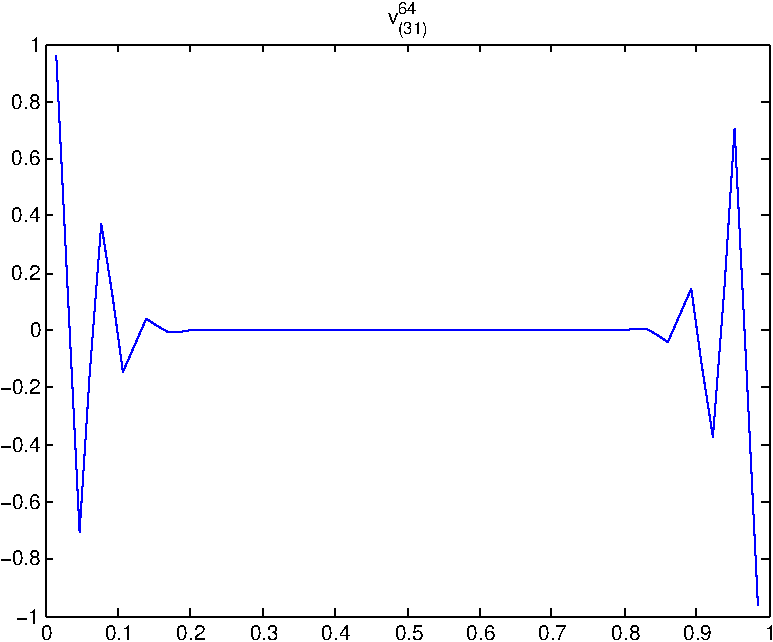
\includegraphics[width=3cm]{images/gauss_v64_31.pdf} & 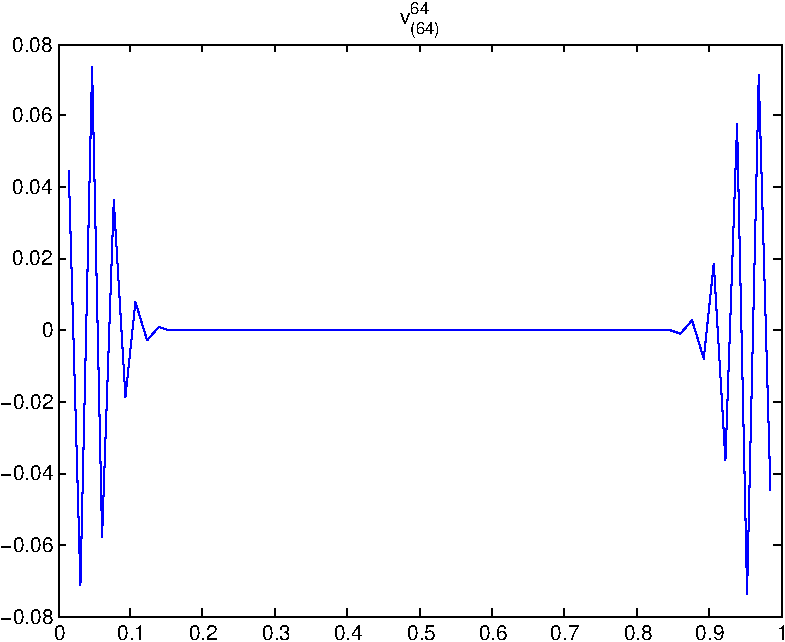
\includegraphics[width=3cm]{images/gauss_v64_64.pdf}
  \end{tabular}
  \caption{Eigenfunctions of $R_G$ when $n=64$ ($h=1/65$).}
 \end{figure}
\end{frame}

\begin{frame}{Gauss-Seidel Spectrum II}
 \begin{figure}
  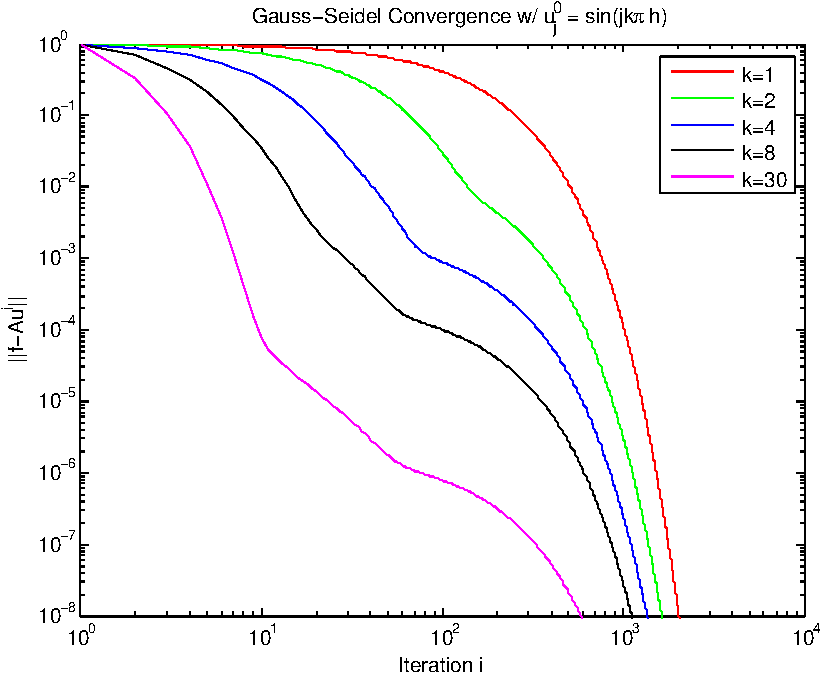
\includegraphics[width=6cm]{images/gaussConvergence_freq.pdf}
  \caption{Unlike Jacobi, Gauss-Seidel is quite effective on high-frequency
           errors.}
 \end{figure}
\end{frame}

\begin{frame}{Damped Jacobi I}
 \begin{itemize}
  \item The Jacobi iteration matrix $R_J$ has eigenvalues
        $\mu_i^h = \cos(i \pi h)$ corresponding to eigenfunctions that are
        sinusoids with normalized frequency $ih$.
  \item Again, this means the low- and high-frequency components of the error
        remain relatively unchanged from iteration to iteration, and are the
        limiting factor in the convergence of the Jacobi method.
  \item What if we could manipulate $R_J$ to get better convergence for some
        of those frequencies?
  \item $R_J(\omega) \defeq (1-\omega) I + \omega R_J$.
  \item This is called \textbf{damping}.
  \item In this case, we have $\mu_i^h(\omega) = 1 - \omega + \omega \cos(i \pi h)$.
  \item If we are concerned about the high frequences, then it suffices to
        consider $i \pi h \approx \pi/2$ and $i \pi h \approx \pi$. We call the corresponding
        eigenvalues $\mu_\text{mid}$ and $\mu_\text{high}$.
 \end{itemize}
\end{frame}

\begin{frame}{Damped Jacobi II}
 \begin{itemize}
  \item $\mu_\text{mid} \approx 1-\omega$, $\mu_\text{high} \approx 1-2\omega$.
  \item If we choose $\omega=2/3$, then that reduces the magnitude of the mid
        and high-frequency eigenvalues to $1/3$, leaving the low-frequency
        eigenvalues relatively unchanged.
  \begin{figure}
   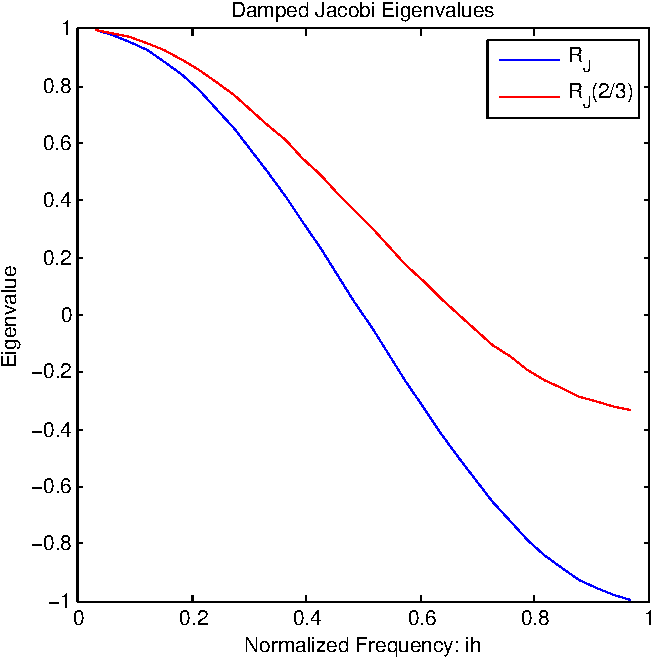
\includegraphics[width=6cm]{images/dampedJacobi.pdf}
  \end{figure}
 \end{itemize}
\end{frame}

\begin{frame}{Damped Gauss-Seidel}
 \begin{itemize}
  \item We can also apply damping to the Gauss-Seidel iteration.
  \begin{align}
   R_G(\omega) = (1-\omega)I + \omega R_J.
  \end{align}
  \item Since $\mu_i^h = \cos^2(i\pi h)$, $\mu_i^h(\omega) = 1 - \omega + \omega \cos^2(i\pi h)$.
  \item Notice that $0 \leq \omega \leq 2$ gives a spectral radius under 1 (convergence).
  \item This iteration with $\omega > 1$ is called
        \textbf{Successive Over-Relaxation} (SOR).
 \end{itemize}
\end{frame}

\begin{frame}{Section Conclusion}
 We have learned:
 \begin{enumerate}
  \item The Jacobi method is a simple solver, but can be \textbf{slow} to converge,
        especially on \textbf{high-frequency} errors.
  \item Gauss-Seidel converges \textbf{twice as fast} as the Jacobi method, and
        performs much better on high-frequency errors.
  \item Both of them can be \textbf{damped} to achieve somewhat better performance.
  \item Both have \textbf{poor performance} on \textbf{low-frequency} errors, which gets
        worse with increasing problem size.
 \end{enumerate}
\end{frame}

\section{Nested Iteration}%====================================================

\begin{frame}{Motivation}
 \begin{itemize}
  \item To speed up a linear solver, we need a good initial estimate $u_0$.
  \item How can we easily compute a good $u_0$?
  \item If the system has an underlying geometric structure, then we can talk
        about the system at different resolutions.
  \item In this case, we can solve the low-resolution versions of the system
        more easily than the full-resolution system since the problem size
        becomes smaller.
  \item Suppose we can solve for a coarse solution $u^{2h}$. Then, a good $u_0$
        may be the upsampled version $I_{2h}^hu^{2h}$.
  \item This strategy lends itself to recursion.
  \item This basic idea is called \textbf{nested iteration}.
 \end{itemize}
\end{frame}

\begin{frame}{Coarse Grids I}
 \begin{itemize}
  \item The reason we can solve our problem better on coarse grids is two-fold:
  \begin{enumerate}
   \item The system has fewer variables.
   \item Relaxation converges faster on small grids (remember $\rho(R_J)=1-O(h^2)$).
  \end{enumerate}
  \item How do we get coarse systems?
  \item We let $I_h^{2h}$ be a linear operator that maps a fine-grid vector $u^{h}$
        to a coarse grid vector $u^{2h}$, and $I_{2h}^h = (I_h^{2h})^T$ be the reverse
        mapping.
  \item A typical choice is the \textbf{full-weighting} operator:
  \begin{align}
   u_i^{2h} &= u_{2i-1}^h/4 + u_{2i}^h/2 + u_{2i+1}^h/4
  \end{align}    
 \end{itemize}
\end{frame}

\begin{frame}{Coarse Grids II}
 \begin{itemize}
  \item Then, we can consider solutions to
  \begin{align}
   I_h^{2h}Au^h=I_h^{2h}f^h.
  \end{align}
  \item However, this is over-determined, so we restrict our search to
        coarse-grid interpolants $u^h=I_{2h}^hu^{2h}$:
  \begin{align}
   I_h^{2h}AI_{2h}^hu^{2h}=I_h^{2h}f^h.
  \end{align}
  \item $A^{2h} \defeq I_h^{2h}AI_{2h}^h$ is the coarse system.
  \item Of course we can keep repeating this to get $A^{4h}$ and so on.
  \item So, supposing we can exactly solve, say, $u^{16h}$, then we can get
        an initial approximation $u_0^h = I_{2h}^hI_{4h}^{2h}\ldots I_{16h}^{8h} u^{16h}$.
  \item This is good if we have no guess, but what can we do when we are already
        \textit{given} $u_0^h$?
 \end{itemize}
\end{frame}

\begin{frame}{Nested Estimation of Error}
 \begin{itemize}
  \item Recall from \hyperlink{relaxation1}{\beamergotobutton{relaxation}} that
        iterating on $Au=f$ with an arbitrary guess $u_0$
        is the same as iterating on $Ae=r$ with an initial guess $e_0=0$.
  \item So, when $u_0$ is given, we need to think of approximating the error
        and using it to correct $u$ starting with the na\"{\i}ve guess of $0$.
  \item To get an approximate answer for $e$, we can use our nested iteration
        idea, then do the correction.
  \item The modification is subtle, but important.
        \begin{algorithmic}[1]
         \State $r^h \gets f^h - A^hu^h$
         \State $r^{2h} \gets I_h^{2h} r^h$
         \State Estimate $A^{2h}e^{2h}=r^{2h}$ for $e^{2h}$ using $e_0^{2h}=0$.
         \State $u^h \gets u^h + I_{2h}^he^{2h}$
        \end{algorithmic}
 \end{itemize}
\end{frame}

\begin{frame}{Analyzing Nested Iteration}
 \begin{itemize}
  \item Note that this structure lends itself to recursion to get the error
        estimate, operating on progressively coarser grids $4h$, $8h$, and so on.
  \item How good is this strategy?
  \item Notice that if the error is \textit{smooth} ($e^h \approx I_{2h}^{h}e^{2h}$),
        then this should work very well since nothing is lost by solving on
        the coarse grid.
  \item But, if the error is not smooth, then we gain nothing.
  \item \textit{Wait a minute!} Nested iteration works well when the error
        is smooth, and relaxation works well when the error is oscillatory (rough).
  \item The two methods are complementary, so can we combine them to get the
        \textbf{ultimate} solver?
 \end{itemize}
\end{frame}

\section{Basic Multigrid Methods}%=============================================

\begin{frame}{V-cycle}
 \begin{algorithmic}[1]
  \Function{vcycle}{$u^i$,$f^i$,$\nu_1$,$\nu_2$}
  \If{$i=1$}
   \Return \textit{exact} solution $u^i$
  \EndIf
  \State \textit{pre-relaxation:} Relax on $A^i\mathbf{u}^i = f^i$ $\nu_1$ times.
  \State $r^i \gets f^i - A^iu^i$ (compute residual)
  \State $e^{i-1} \gets$ VCYCLE($e^{i-1} = 0$,$I_i^{i-1}r^i$) (estimate correction)
  \State $u^i \gets u^i + I_{i-1}^i e^{i-1}$. (apply correction)
  \State \textit{post-relaxation:} Relax on $A^i\mathbf{u}^i = f^i$ $\nu_2$ times.
  \State \Return $u^i$
  \EndFunction
 \end{algorithmic}

 \begin{itemize}
  \item Base case: solve the coarsest problem directly by some means.
  \item Do Jacobi or Gauss-Seidel relaxation to get rid of high-frequency errors.
  \item Solve for the coarse correction by recursion on next coarser level.
  \item Upsample and apply coarse correction.
  \item Smooth the new estimate by relaxation.
 \end{itemize}
\end{frame}

\begin{frame}
 \begin{figure}
  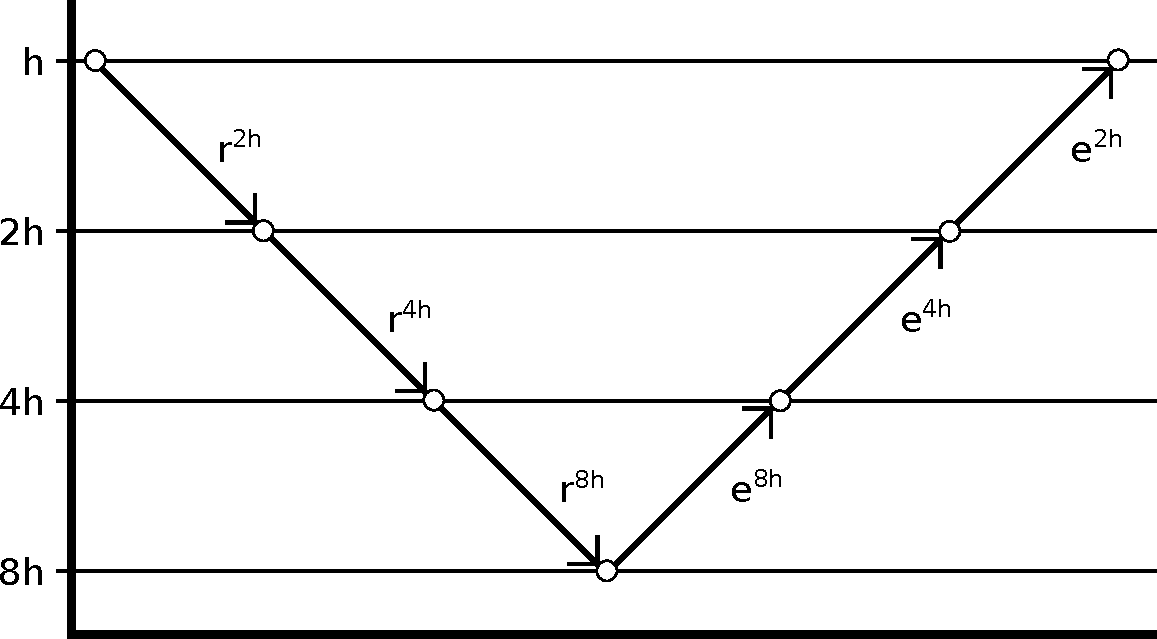
\includegraphics[width=7cm]{images/vcycleSchedule.pdf}
  \caption{V-cycle schedule. The reason for the name becomes clear.}
  \label{fig:vcycleSchedule}
 \end{figure}

 \begin{itemize}
  \item Fig. \ref{fig:vcycleSchedule} gives a visualization for the v-cycle schedule.
  \item Each level computes a coarse residual for the next lower level.
  \item Once the residual reaches the coarsest level, errors are computed and
        passed to next finer level.
 \end{itemize}

\end{frame}

\section{Analysis}%============================================================

\section{Recent Work}%=========================================================

\section*{Extra Material}%=====================================================

\begin{frame}[label=gaussSeidelProof]{Gauss-Seidel Spectrum I}
 % NOTE: have to split up theorem and proof, and not use the proof environment
 %       because beamer does not properly split it across slides.
 \begin{theorem}
  $\mu_i^h = \cos^2(i\pi h), \; v_{(i)j}^h = \cos^j(i\pi h)\sin(ij\pi h)$
 \end{theorem}
  \begin{beamercolorbox}{titlelike}
   Proof
  \end{beamercolorbox}
  
  Note that $Rv=\mu v$ is:
  \begin{align}
   \mu\left(2 \begin{bmatrix}v_1\\ \vdots \\ v_{n-1} \\ v_n \end{bmatrix} - \begin{bmatrix} 0 \\ v_1 \\ \vdots \\ v_{n-1} \end{bmatrix} \right) = \begin{bmatrix}v_2\\ \vdots \\ v_n \\ 0\end{bmatrix}.
  \end{align}

  So, it is sufficient to show that
  \begin{align}
   v_{(i)j}/\mu_i = 2v_{(i)j-1} - v_{(i)j-2}. \nonumber
  \end{align}
  First, note the identity:
  \begin{align}
   \sin(u)+\sin(v) = 2\sin\left(\frac{u+v}{2}\right)\cos\left(\frac{u-v}{2}\right) \nonumber
  \end{align}
\end{frame}
\begin{frame}{Gauss-Seidel Spectrum II}
  So, we have
  \begin{align}
   \sin(ji\pi h) + \sin((j-2)i\pi h) = 2 \sin\left( (j-1)i\pi h \right) \cos\left( i\pi h \right). \nonumber
  \end{align}
  This implies
  \begin{align}
   \sin(ji\pi h) = \cos(i \pi h) \sin((j-1)i\pi h) - \sin((j-2)i\pi h). \nonumber
  \end{align}
  Then, we get
  \begin{align}
   \cos^{j-2}(i\pi h)\sin(ji\pi h) =& \; 2\cos^{j-1}(i \pi h) \sin((j-1)i\pi h) \nonumber \\
                                      &- \cos^{j-2}\sin((j-2)i\pi h), \nonumber
  \end{align}
  which is the original recurrence relation.
  So, the proposed eigenpairs describe the spectrum.
  \qed \\
  \hyperlink{gaussSeidel}{\beamergotobutton{Back}}
\end{frame}

% References ==================================================================
\begin{frame}[allowframebreaks]
 \nocite{*}
 \frametitle{References}
 \bibliographystyle{amsalpha}
 \bibliography{multigridrefs.bib}
\end{frame}

\end{document}
